% vim: set textwidth=78 autoindent:

\section{Uso dei Plugin Core QGIS}\label{sec:core_plugins}\index{plugins!core}

% when the revision of a section has been finalized, 
% comment out the following line:
%\updatedisclaimer

QGIS al momento contiene 17 plugins di base che possono essere caricati tramite
il Plugin Manager.
La tabella \ref{tab:core_plugins} mostra una lista dei plugins di base, insieme
ad una descrizione del loro scopo e l'icona che viene mostrata nella barra dei
menù.\footnote{Il Plugin MapServer
Export Plugin ed il Plugin Installer Plugin sono Plugins Python esterni,
ma sono parte delle fonti QGIS e automaticamente caricati e selezionabili nel QGIS Plugin Manager.}

% minipage is needed to appear the footnote under the table
% SH
\begin{minipage}{\textwidth}
\begin{table}[H]
\centering
\caption{QGIS Core Plugins}\label{tab:core_plugins}\medskip
\small
 \begin{tabular}{|l|l|p{4in}|}
\hline \textbf{Icon} & \textbf{Plugin} & \textbf{Description}\\
\hline

\includegraphics[width=0.6cm]{delimited_text}
 & Aggiungi layer testo delimitato \index{plugins!Testo delimitato} & Carica e mostra files di testo delimitato contenenti coordinate x,y\\
\hline

\includegraphics[width=0.6cm]{coordinate_capture}
 & Cattura Coordinate \index{plugins!Cattura coordinate}& Cattura le coordinate del mouse
usando SRS diverso\\
\hline 
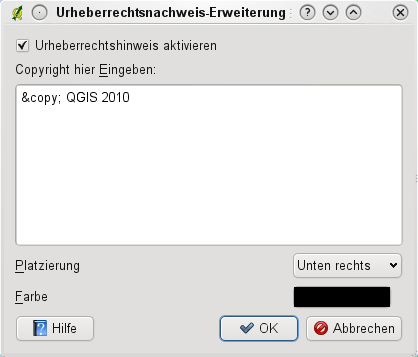
\includegraphics[width=0.6cm]{copyright_label}
 & Etichetta di copyright \index{plugins!Etichetta di copyright}& Disegna una Etichetta di copyrightcon informazioni\\
\hline 

\includegraphics[width=0.6cm]{dxf2shp_converter}
 & DXF2Shape Convertitore \index{plugins!Convertitore DXF2Shape}& Converte da formato DXF a SHP\\
\hline

\includegraphics[width=0.6cm]{gps_importer}
 & Strumenti GPS \index{plugins!gps}& Strumenti per caricare e importare dati GPS\\
\hline

\includegraphics[width=0.6cm]{grass}
 & GRASS \index{plugin!strumenti grass} & Attiva il potente strumentario GRASS\\
\hline
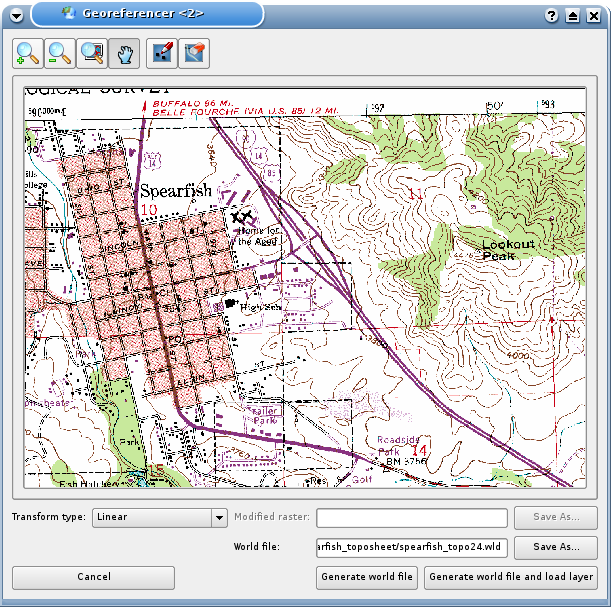
\includegraphics[width=0.6cm]{georeferencer}
 & Georeferenziatore \index{plugin!georeferenziatore} & Aggiunge proiezioni ai file raster\\
\hline

\includegraphics[width=0.6cm]{grid_maker}
 & Creatore di Griglia \index{plugins!Creatore di Griglia}& Crea una griglia latitudine/longitudine e la salva come  shape\\
\hline

\includegraphics[width=0.6cm]{interpolation}
& Plugin di Interpolazione  \index{plugins!Interpolazione}& Interpolazione basata sui vertici di un layer vettoriale\\
\hline

\includegraphics[width=0.6cm]{mapserver_export}
& Plugin MapServer Export \index{plugins!MapServer Export}& Esporta un progetto salvato QGIS
in un file mappa MapServer \\
\hline
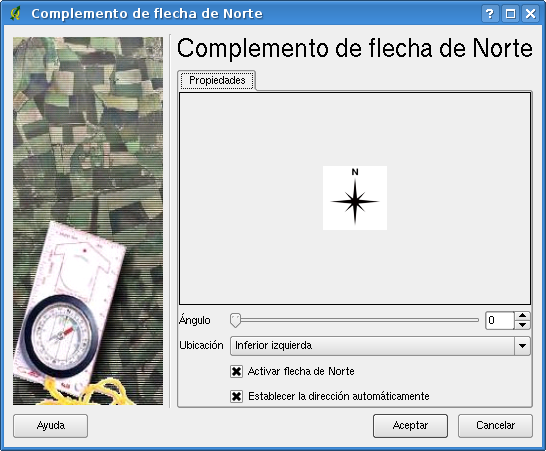
\includegraphics[width=0.6cm]{north_arrow}
& Freccia Nord \index{plugins!Freccia Nord}& Mostra una freccia che indica il nord sovrapposta alla mappa\\
\hline

\includegraphics[width=0.6cm]{ogr_converter}
 & Convertitore di layer OGR \index{plugins!Convertitore OGR} & Traduce i layer vettoriali tra formati supportati OGR\\
\hline

\includegraphics[width=0.6cm]{plugin_installer}
 & Istallatore di Plugin  \index{plugins!Istallatore di Plugin} & Scarica e istallai plugin QGIS python\\
\hline

\includegraphics[width=0.6cm]{spiticon}
 & SPIT \index{plugins!spit}& Strumento di importazione di file shape in PostgreSQL/PostGIS \\
\hline

\includegraphics[width=0.6cm]{quick_print}
 & Stampa veloce \index{plugins!Stampa veloce}& Stampa rapidamente una mappa con sforzo minimo \\
\hline
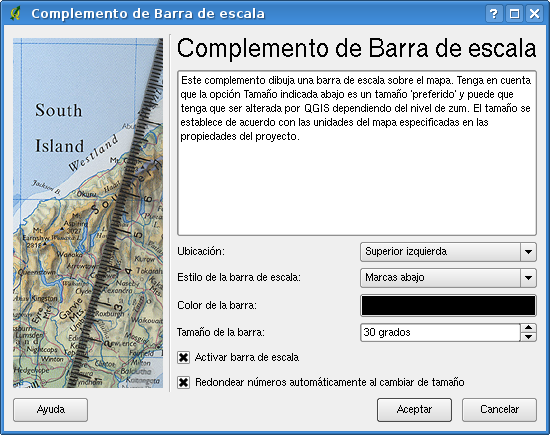
\includegraphics[width=0.6cm]{scale_bar}
 & Barra di Scala \index{plugins!barra di scala}& Disegna una barra di scala\\
\hline

\includegraphics[width=0.6cm]{mIconAddWfsLayer}
 & WFS & Carica e mostra un layer WFS\\
\hline
\end{tabular}
\end{table}
\end{minipage}

\normalsize

\begin{Tip}\caption{\textsc{Impostazioni dei plugin salvate nel progetto}}\index{Impostazione dei plugins}
\qgistip{Quando si salva un progetto .qgs, qualsiasi cambiamento fatto ai plugin  Freccia Nord, Barra di Scala e Etichetta di Copyright saranno salvate nel progetto e ripristinate la prossima volta che si apre il progetto.}
\end{Tip}
